% Copyright 2016-2023 - Julien TREBOSC, Bas van Meerten and Wouter Franssen
%
%This file is part of ssNake.
%
%ssNake is free software: you can redistribute it and/or modify
%it under the terms of the GNU General Public License as published by
%the Free Software Foundation, either version 3 of the License, or
%(at your option) any later version.
%
%ssNake is distributed in the hope that it will be useful,
%but WITHOUT ANY WARRANTY; without even the implied warranty of
%MERCHANTABILITY or FITNESS FOR A PARTICULAR PURPOSE.  See the
%GNU General Public License for more details.
%
%You should have received a copy of the GNU General Public License
%along with ssNake. If not, see <http://www.gnu.org/licenses/>.

\documentclass[11pt,a4paper]{article}
% Copyright 2016 - 2017 Bas van Meerten and Wouter Franssen
%
%This file is part of ssNake.
%
%ssNake is free software: you can redistribute it and/or modify
%it under the terms of the GNU General Public License as published by
%the Free Software Foundation, either version 3 of the License, or
%(at your option) any later version.
%
%ssNake is distributed in the hope that it will be useful,
%but WITHOUT ANY WARRANTY; without even the implied warranty of
%MERCHANTABILITY or FITNESS FOR A PARTICULAR PURPOSE.  See the
%GNU General Public License for more details.
%
%You should have received a copy of the GNU General Public License
%along with ssNake. If not, see <http://www.gnu.org/licenses/>.

\usepackage[british]{babel}
\usepackage{graphicx,booktabs,listings,amsmath,pgfplots,pgfplotstable}
\usepackage[small,bf,nooneline]{caption}
\usepackage{subcaption}
\usepackage[sort&compress,numbers]{natbib}
\usepackage{tikz}
\usepackage{mathtools}
\usepackage[nottoc]{tocbibind}%adds bibliography to table of contents.
\graphicspath{{./images/}}
%\setlength{\textwidth}{453pt} %597 pt is the a4 paperwidth. Minus 2 in margin. 72 pt = 1 in
%\setlength{\hoffset}{-\oddsidemargin}
%\setlength{\voffset}{-30pt} %
%\setlength{\textheight}{651 pt} %a4 height 845 pt minus 2* total headheight. In this case 2*88pt
%% examine margines via the layout package. Use command \layout{} in document to draw a picture.
%\setlength{\parindent}{0.5 cm}
%\setlength{\parskip}{0 cm}
\usepackage[left=82pt,right=82pt,top=95pt,bottom=95pt,footnotesep=0.5cm]{geometry}
%\setlength{\headheight}{14pt}

%define colours--------------------
%dark
\usepackage{xcolor}
\definecolor{MyGrayD}{RGB}{1,1,1}
\definecolor{MyRedD}{RGB}{237,45,46}
\definecolor{MyGreenD}{RGB}{0,140,71}
\definecolor{MyBlueD}{RGB}{24,89,169}
\definecolor{MyOrangeD}{RGB}{243,125,34}
\definecolor{MyPurpleD}{RGB}{102,44,145}
\definecolor{MyBrownD}{RGB}{161,29,32}
\definecolor{MyPinkD}{RGB}{179,56,147}
%normal
\definecolor{MyGray}{RGB}{114,114,114}
\definecolor{MyRed}{RGB}{241,89,95}
\definecolor{MyGreen}{RGB}{121,195,106}
\definecolor{MyBlue}{RGB}{89,154,211}
\definecolor{MyOrange}{RGB}{249,166,90}
\definecolor{MyPurple}{RGB}{158,102,171}
\definecolor{MyBrown}{RGB}{205,112,88}
\definecolor{MyPink}{RGB}{215,127,179}
%light
\definecolor{MyGrayL}{RGB}{204,204,204}
\definecolor{MyRedL}{RGB}{242,174,172}
\definecolor{MyGreenL}{RGB}{216,228,170}
\definecolor{MyBlueL}{RGB}{184,210,235}
\definecolor{MyOrangeL}{RGB}{242,209,176}
\definecolor{MyPurpleL}{RGB}{212,178,211}
\definecolor{MyBrownL}{RGB}{221,184,169}
\definecolor{MyPinkL}{RGB}{235,191,217}
%----------------------------------

%Figure ref with hyperref
\newcommand{\fref}[1]{\hyperref[#1]{Figure \ref*{#1}}}
\newcommand{\sref}[1]{\hyperref[#1]{Section \ref*{#1}}}
\newcommand{\tref}[1]{\hyperref[#1]{Table \ref*{#1}}}

%Makes a new command for figures with input values: filename, width(times linewidth),
% caption and label.
\newcommand{\onefigure}[4]{
\setlength{\captionwidth}{#2\linewidth}
\begin{figure}
\includegraphics[width=#2\linewidth]{#1}
\centering
\parbox{\linewidth}{\caption{#3}
\label{#4}}
\end{figure}
}

%Makes a new command for tikz figures with input values: tikz commands, 
% caption and label.
\newcommand{\onetikz}[3]{
\settowidth{\captionwidth}{#1}
\ifthenelse{\lengthtest{\captionwidth<0.7\linewidth}}{\setlength{\captionwidth}{0.7\linewidth}}{}

\begin{figure}
\centering
#1
\centering
\parbox{\linewidth}{\caption{#2}
\label{#3}}
\end{figure}
}

%Makes a new command for two figures next to each other with input values: filename1, caption1, label1,filename2, caption2 and label2. Figure width is set to 0.47\linewidth and the space between the figures is filled with \hfill so the sides of the figures align with to edge of the line.
\newcommand{\twofigure}[6]{
\setlength{\captionwidth}{\linewidth}
\begin{figure*}[ht!]
\begin{minipage}[t]{0.47\linewidth}
\includegraphics[width=\linewidth]{#1}
\centering
\caption{#2}
\label{#3}
\end{minipage}
\hfill
\begin{minipage}[t]{0.47\linewidth}
\centering
\includegraphics[width= \linewidth]{#4}
\centering
\caption{#5}
\label{#6}
\end{minipage}
\end{figure*}
}


%Makes a new command for a table with caption witdh equal to the total table width. Input: tabular, caption and label. Example:
%\onetable{
%\begin{tabular}{ccc}
%a&b&c\\
%\hline
%1&1&1\\
%1&1&1\\
%1&1&1\\
%\end{tabular}
%{The caption.}
%{tab:table1}
%}
\newcommand{\onetable}[3]{
\settowidth{\captionwidth}{#1}
\ifthenelse{\lengthtest{\captionwidth<0.7\linewidth}}{\setlength{\captionwidth}{0.7\linewidth}}{}
\begin{table}
\caption{#2}
\vspace{-0.24cm} %Puts caption close to toprule
\label{#3}
\centering
#1
\end{table}
}

%Makes a long table with captionwidth equal to tablewidth. It takes the following arguments:
%1: Column specifier (e.g. cccc)
%2: Caption
%3: Label
%4: First head (i.e. first row of regular table)
%5: Head of consecutive pages
%6: Foot of pagebreak
%7: Lastfoot (e.g. \midrule)
%8: Body of table
\newcommand{\onelongtable}[8]{
\begin{center}
\settowidth{\captionwidth}{
\begin{tabular}{#1}
#4
#8
\end{tabular}} % This ends the captionwidth part. Next comes the real table.

\begin{longtable}{#1}
\caption{#2}\\
\vspace{-0.74cm} %Puts caption close to toprule
\label{#3}\\

#4
\endfirsthead

#5
\endhead

#6
\endfoot

#7
\endlastfoot

#8
\end{longtable}
\end{center}}




%1:pgfplots code
%2:width
%3:caption
%4:label
\newcommand{\pgfplotsfigure}[4]{
\pgfplotsset{width=#2\linewidth}
\setlength{\captionwidth}{#2\linewidth}
\begin{figure}[t]
\centering
#1
\centering
\parbox{\linewidth}{\caption{#3}
\label{#4}}
\end{figure}
}


\usepackage[bitstream-charter]{mathdesign}
\usepackage[T1]{fontenc}
\usepackage[protrusion=true,expansion,tracking=true]{microtype}
\pgfplotsset{compat=1.7,/pgf/number format/1000 sep={}, axis lines*=left,axis line style={gray},every outer x axis line/.append style={-stealth'},every outer y axis line/.append style={-stealth'},tick label style={font=\small},label style={font=\small},legend style={font=\footnotesize}}
\usepackage{colortbl}
\usetikzlibrary{calc}

%Set section font
\usepackage{sectsty}
\allsectionsfont{\color{black!70}\fontfamily{SourceSansPro-LF}\selectfont}
%--------------------


%Set toc fonts
\usepackage{tocloft}
%\renewcommand\cftchapfont{\fontfamily{SourceSansPro-LF}\bfseries}
\renewcommand\cfttoctitlefont{\color{black!70}\Huge\fontfamily{SourceSansPro-LF}\bfseries}
\renewcommand\cftsecfont{\fontfamily{SourceSansPro-LF}\selectfont}
%\renewcommand\cftchappagefont{\fontfamily{SourceSansPro-LF}\bfseries}
\renewcommand\cftsecpagefont{\fontfamily{SourceSansPro-LF}\selectfont}
\renewcommand\cftsubsecfont{\fontfamily{SourceSansPro-LF}\selectfont}
\renewcommand\cftsubsecpagefont{\fontfamily{SourceSansPro-LF}\selectfont}
%--------------------

%Define header/foot
%\usepackage{fancyhdr}
%\pagestyle{fancy}
%\fancyhead[LE,RO]{\fontfamily{SourceSansPro-LF}\selectfont \thepage}
%\fancyhead[LO,RE]{\fontfamily{SourceSansPro-LF}\selectfont \leftmark}
%\fancyfoot[C]{}
%--------------------

%remove page number from first chapter page
%\makeatletter
%\let\ps@plain\ps@empty
%\makeatother
%----------------------

\usepackage[hidelinks,colorlinks,allcolors=black, pdftitle={Advanced MQMAS processing in ssNake},pdfauthor={Julien TRÉBOSC}]{hyperref}

\interfootnotelinepenalty=10000 %prevents splitting of footnote over multiple pages
\linespread{1.2}

\title{\color{black}\fontfamily{SourceSansPro-LF}\bfseries Advanced MQMAS processing in ssNake}
\author{}
\date{\color{black}\fontfamily{SourceSansPro-LF}\bfseries \today}


\begin{document}
%\newgeometry{left=72pt,right=72pt,top=95pt,bottom=95pt,footnotesep=0.5cm}
\microtypesetup{protrusion=true} % enables protrusion

\maketitle

%%%%%%%%%%%%%%%%%%%%%%%%%%%%%%%%%%%%%%%%%%%%%%%%%%%%%%%%%%%%%%%%%%%%%%%%%%%%%%%%%%%%%%%%%%%%%%%%%%%%
\section{Introduction}
This tutorial will make a review of MQMAS experiment principles and will present several ways to process and fit 
Multiple Quantum Magic Angle spinning (MQMAS) NMR data using ssNake.
We will present several representation of MQMAS (or STMAS) spectra: unsheared (3Q/SQ)/sheared/Q-sheared.
The tutorial delivered with the ssNake program is considered as prior knowledge and having done MQMAS tutorial is advized.
If you have not yet studied this, please do so before continuing with these examples.

This tutorial is assuming ssNake version 1.5 to be used. There is a change on sign of shearing and scaling with respect to 
previous versions depending on spin I and MQ level. ssNake v1.5 calculations for shearing and scale assume an evolution on 
$-pQ$ ($p=$3, 5, 7 or 9 for MQMAS and $p= 1 or 2$ for STMAS and DQ-STMAS. While previous versions assume a coherence pathway 
such that quadrupolar echo is shifting towards positive $t_2$ time.

%%%%%%%%%%%%%%%%%%%%%%%%%%%%%%%%%%%%%%%%%%%%%%%%%%%%%%%%%%%%%%%%%%%%%%%%%%%%%%%%%%%%%%%%%%%%%%%%%%%%
\section{MQMAS principles}
MQMAS is a 2D experiment for half-integer quadrupolar nuclei which is used to obtain isotropic information from nuclei 
broadened by the second order quadrupole interaction. This allows the separation of multiple overlapping quadrupolar 
sites on the basis of their `isotropic' value (which is a combination of the isotropic chemical shift, and the isotropic 
quadrupolar shift, which is also called the quadrupolar induced shift). 

The experiment can be quite difficult to process.
Not because of the complication of the steps involved, but due to the large number of different MQMAS experiments and the various ways to process these.
This advanced tutorial will give several examples of MQMAS processing in various cases and give hints on parameters that must be
considered to run processing in the proper way.
Moreover, it will explain how to simulate different kind of processing.

The principle of MQMAS is to correlate $-pQ$ coherence ($p=3$, 5, 7 or 9) during $t_1$ evolution with the observable $-1Q$ 
coherence. The total signal phase evolution during $t_1$ and $t_2$ is 
$$\omega_Q(-pQ) \cdot t_1 + \omega_Q(-1Q) \cdot t_2$$
for quadrupolar interaction and
$$\omega_{CS}(-pQ) \cdot t_1 + \omega_{CS}(-pQ) \cdot t_2$$
for chemical shift interaction.

The dephasing can cancel at a point in $t_2$ evolution when $t_2 = - {\omega(-pQ) \over \omega(-pQ)} t_1$.
The ratio of dephasing occuring during $-pQ$ and $-1Q$ is
$$R={\omega_Q(-pQ) \over \omega_Q(-1Q)}$$
for the second order quadrupolar interaction and
$${\omega_{CS}(-pQ) \over \omega_{CS}(-1Q)} = p $$
for the chemical shift interaction.

The reason for MQMAS to be working is that ratios R and p are independant of $C_Q$/$\eta_Q$ and chemical shift 
amplitudes respectively, and these ratio are different ($R \neq p$) which allows to separate their contributions along 
different axes.
Depending on p and spin S, the ratio R of quadrupolar dephasing can be positive or negative. For chemical shift the ratio is $+p$.
A negative ratio means that dephasing in $t_1$ and $t_2$ are canceling leading to the formation of an echo at positive time 
($t_2 = - R \cdot t_1$).
A positive ratio means that dephasings are cumulative in $t_1$ (evolution on $-pQ$) and $t_2$ (evolution on $-1Q$). 
The echo is shifting to negative $t_2$. Note that a positive R will result in a spectrum correlation with 
slope $F_1=R\cdot F_2$, but a quadrupolar echo that shifts with $t_2 = -R \cdot t_1$.

Depending on the dominating interaction one can observe the formation of an echo at position $t_2 = -R \cdot t_1$ if 
the quadrupolar interaction is strong or at $t_2 = -3 \cdot t_1$ if chemical shift distribution is dominating.

Z-Filter MQMAS is acquired in hyper-complex mode (for example State): echo and anti-echo are recorded simultaneously so a signal
is always observed at positive $t_2$. The way quadrature is implemented (within the pulse sequence and hardware) will select 
the $\pm pQ$ pathway (more often the expected $-pQ$).
A full echo MQMAS only selects one pathway. It can be $\pm pQ$ depending on the pulse sequence implementation and on the 
requirement to have signal in positive acquisition time ($t_2$). Indeed very often the pulse sequence will select the pathway
for which an echo shifts towards increasing $t_2$ times ($R < 0$).
If $+pQ$ is selected by the pulse sequence, then one will need to perform a Complex conjugate operation on D1 time domain, 
or a flip Left/Right operation on D1 frequency domain to flip the spectrum (indeed $\omega(pQ) = -\omega(-pQ)$).

Therefore, apodization should be done along $-R$ axis (or $\pm$R axes for Z-Filter MQMAS when echo and anti-echo are selected).
In some experiments the dominating interaction is chemical shift distribution. In that case, the echo is mostly appearing 
at $t_2 = -p \cdot  t_1$. Then the slope for shifting should be $\pm$p. Eventualy one should look at the FID to determine the best
apodization and slope.


Shearing process aligns the correlation peaks horizontally instead of along the R slope by rolling each column (in D1 dimension). 
Shearing should always be done relative to the carrier frequency to get proper scale (the column at the carrier 
in D2 remains unchanged). In time domain shearing is equivalent to make the quadrupolar echo be positioned
at $t_2=0$ (time when second order quadrupolar dephasings are canceled). 

Once shearing is done, a universal scale can be designed that will make the peaks appear at the same position (in ppm)
whatever p is used (3QMAS, 5QMAS, or even STMAS). There are two way to achieve such scale:
\begin{itemize}
  \item Scale the spectral window (SW).
  \item Scale the carrier and reference frequencies used to calculate ppm scale).
\end{itemize}

When using SW scaling, the spinning sidebands will appear at scaled spinning speed in kHz. When using carrier and 
reference scaling, the spinning sideband separation remains at the spinning speed in kHz, however the Chemical Shift axis 
slope is scaled (due to shearing operation) and is 1 only when both axis are in ppm unit.

\subsection{Split-t1 experiments}
Split-t1 MQMAS experiments are designed to refocus the second order quadrupolar anisotropy at a fix time in D2.
This corresponds to applying a shearing processing operation. It is usually done by defining a delay $\tau$, on $\pm 1Q$ quantum
level, which duration depends on $t_1$ (pQ coherence evolution) such that $\tau = R \cdot t_1$ before the acquisition during $t_2$.

Therefore, one just need to deal with such experiment just the same as a pQMAS experiment. The experiment does not need be sheared, 
and should be scaled as pQMAS experiment with $t_1$ evolution defined as evolution time on $pQ$. 

%%%%%%%%%%%%%%%%%%%%%%%%%%%%%%%%%%%%%%%%%%%%%%%%%%%%%%%%%%%%%%%%%%%%%%%%%%%%%%%%%%%%%%%%%%%%%%%%%%%%
\section{ssNake tools for MQMAS processing}
Note that current ssNake tools assume that the quadrupolar echo is shifting towards 
positive $t_2$ time. For example, for spin 5/2 3QMAS, it will use a ratio $R=19/12$ corresponding to 
$R = {\omega_Q(+3Q) \over \omega_Q(-1Q)}$ that is evolution on $+3Q$ during $t_1$. It will apply the corresponding 
ratio for shearing. Since in that case the spectrum in D1 is reversed, the Scale SW tool will propose to use
a negative factor (-12/17) that will reverse the D1 axis (instead of the data as when using Flip L/R tool or using 
complex conjugate in time domain before FT). 

Fitting of MQMAS will also
The simulation procedure calculate the frequency of $-pQ$ and $-1Q$ for each crystallite. The `Auto' button calculates the 
the shear and Scale SW parameters adequately. 

\section{Data}
In this tutorial we will use several datasets:
\begin{itemize}
\item a Z-filter 3QMAS of 5/2 spin nucleus (${}^{27}$Al).
\item an unconventional split-t1 full echo 3QMAS of 3/2 spin nucleus (${}^{35}$Cl).
\item a Z-filter STMAS recorded with NUS of 3/2 spin nucleus (${}^{87}$Rb).
\end{itemize}


%%%%%%%%%%%%%%%%%%%%%%%%%%%%%%%%%%%%%%%%%%%%%%%%%%%%%%%%%%%%%%%%%%%%%%%%%%%%%%%%%%%%%%%%%%%%%%%%%%%%
\section{Z-Filter MQMAS processing}
First, we will look into the processing of MQMAS data recorded using a Z-Filter experiment (also called three pulse MQMAS).
Note that data recorded with a regular two pulse MQMAS (the standard MQMAS experiment) can be processed in the same way.

Open the `3QMAS-Z' dataset. This is a ${}^{27}$Al 3QMAS experiment of AlPO VPI-5 mesoporous sample. It has been recorded 
in States-TPPI mode on a 18.8~T spectrometer at 20~kHz MAS rate.

Be careful that some information in the dataset may be wrong or unexpected. Especially the carrier and reference frequencies
in dimension D1 may be already scaled (if xfshear has been applied under Topspin) or even correspond to a wrong nucleus. 
In the worst case, the SW could be wrong. This could happen if actual $t_1$ evolution increment (on Bruker this would often 
be parameter IN0) does not correspond to declared spectral window (parameter SW\_h in Bruker).

Processing of the data is performed in the following steps:
\begin{itemize}
  \item Remove digital filter.
  \item Set the view to D1 (sideframe, radiobutton).
  \item Convert the hypercomplex data via Transforms  $\longrightarrow$ Hypercomplex  $\longrightarrow$
   selecting `States-TPPI'.
  \item Set the view back to D2 (sideframe, radiobutton).
  \item Apodize in D2 using a gaussian apodization (50~Hz), with shifting (select `Spin 5/2 3QMAS' which enter a Value or 19/12).
\end{itemize}

Note the shifting option. We chose to shift apodization along the quadrupolar echo slope. But in some spectra, chemical shift 
distribution could be dominant and a slope of 3 would be better. One can also choose a compromise that is a slope in between
the two.

The FID should now look like this:
\begin{center}
%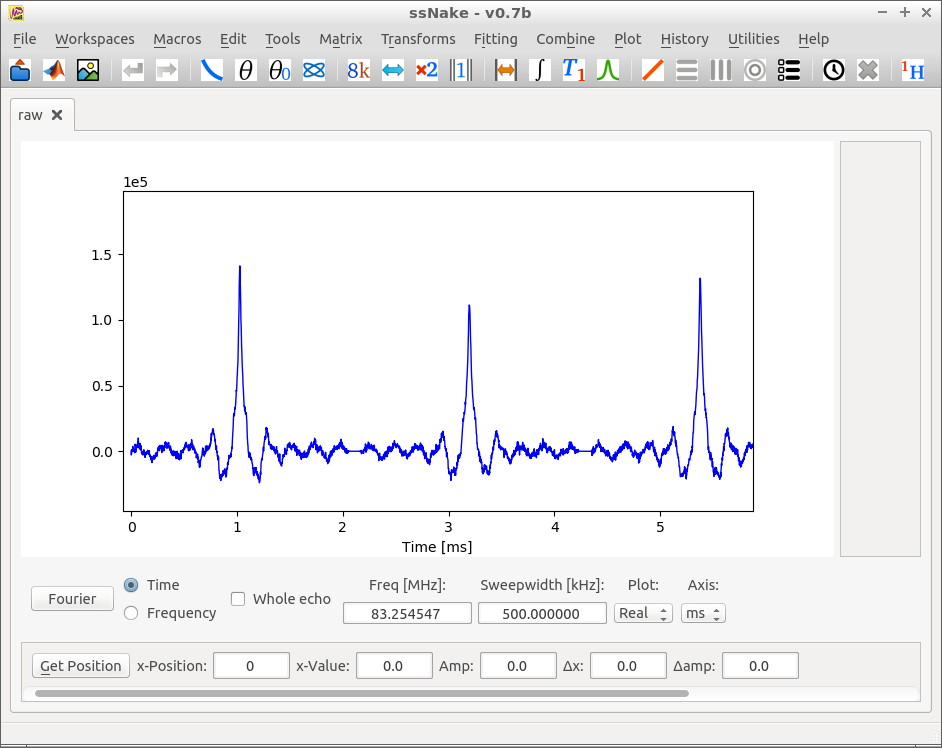
\includegraphics[width=0.8\linewidth]{Figs/Fig1.png}
\end{center}

Continue with the following processing steps.
\begin{itemize}
  \item Zero-fill (Matrix $\longrightarrow$  Sizing) 2048 points. (FID will be shortened).
  \item Fourier Transform D2 (ctrl-F shortcut), and phase the first slice.
  \item Optional baseline correction in D2 (`Tools' $\longrightarrow$ `Baseline Correction') + Hilbert transform or HT
      (`Transform' $\longrightarrow$ `Hilbert Transform'). HT is required after operations that only affect the real part
       but not the imaginary.
  \item Set the view to D1 (in sideframe radiobutton).
  \item Processing of the indirect dimension D1 (zerofilling 512 points, apodizing (50~Hz Lorenztian broadening), Fourier transform, phasing).
\end{itemize}

At that point we have several options for processing\label{choice}:
\begin{itemize}
  \item whether to shear the spectrum.
  \item whether to scale the spectral width or the carrier and reference frequencies in the indirect dimension.
\end{itemize}

\subsection{3Q-1Q representation} \label{_3Q1Q}
First we can choose to represent the spectrum in 3Q-1Q scale. To do that we need to adjust the reference frequency to $3 \cdot Ref - 2 \cdot Car$
where Ref is D2 dimension reference frequency and Car is the carrier frequency in D2 (and D1). Indeed this will ensure that the center 
of the spectrum will correspond to ppm coordinates $(F1, F2)= (p, 3p)$.
First we need to ensure that D1 Carrier and Reference frequencies in D1 correspond to D2. This may not be necessary but as said before
they may not be correct.
Go to menu `Tools' $\longrightarrow$ `Reference' $\longrightarrow$ `Set Reference'. Give name `D2' and validate.
Copy (crtl-C) the carrier frequency shown in D2 dimension. 
Select dimension D1
Paste the Carrier Frequency from D2.
Go to menu `Tools' $\longrightarrow$ `Reference' $\longrightarrow$ `Apply'. Select `D2'.
Go to menu `Tools' $\longrightarrow$ `Reference' $\longrightarrow$ `Set Reference', then apply the operation $3 \cdot Ref - 2 \cdot Car$ for 
the reference frequency (There you can also `Paste' the Carrier frequency that was copied above to write the equation).

This results in the following spectrum:
\begin{center}
%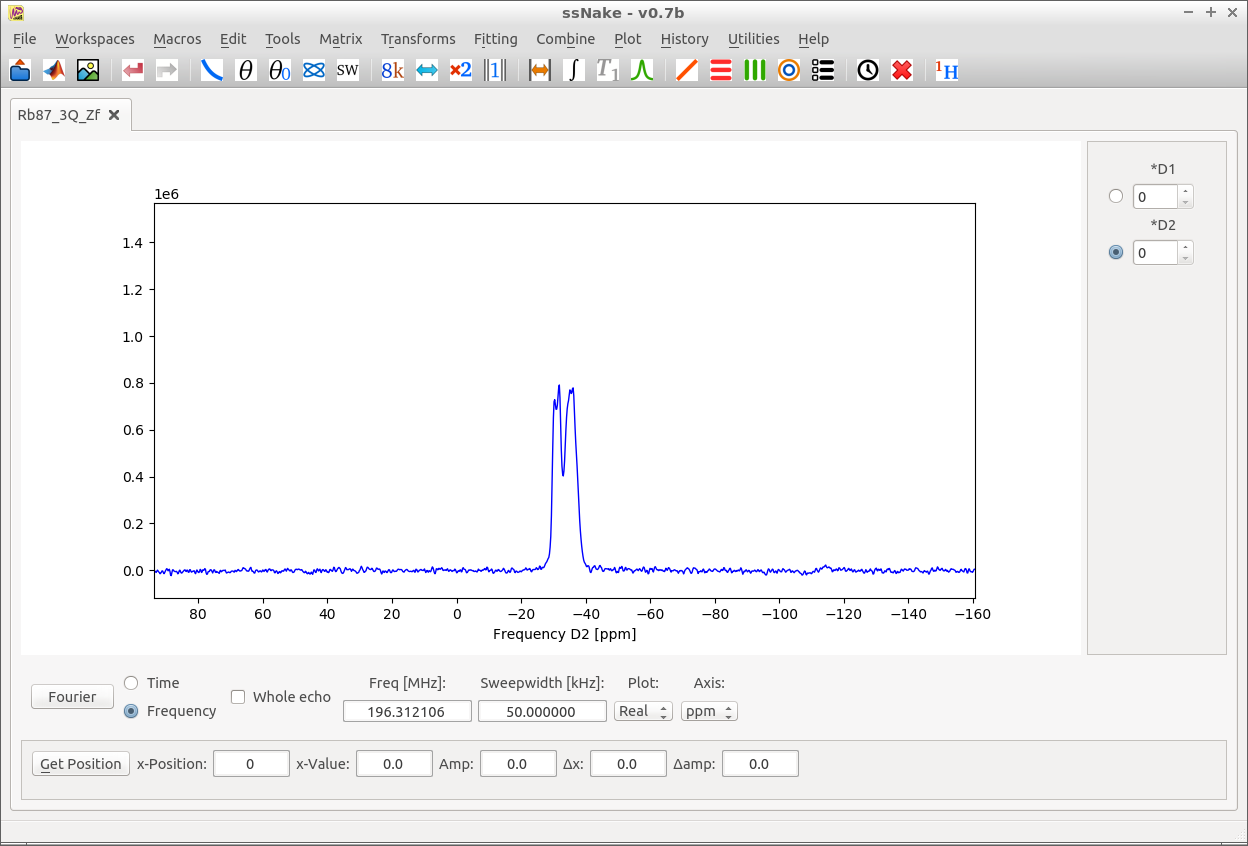
\includegraphics[width=0.8\linewidth]{Figs/Fig2.png}
\end{center}

One can fit such spectrum with MQMAS model. There are 3 sites with main parameters summarized in table \ref{table:AlPO_vpi5_sites}. The fourth site
at about 5~ppm is actually an impurity that will not be considered in the following.

\begin{center}\label{table:AlPO_vpi5_sites}
  \begin{tabular}{c|c c c} 
	 \toprule
	 Site & $\delta_\text{iso}$ [ppm]& $C_\text{Q}$ [MHz] & $\eta_\text{Q}$ \\
	 \midrule
 1 & -10.10      &   3.448     &          0.8992       \\
 2 &  41.74      &   1.274     &          0.4267       \\
 3 &  43.69      &   2.292     &          0.8697       \\
	\bottomrule
  \end{tabular}
\end{center}

Open a MQMAS fitting window (menu `Fitting' $\longrightarrow$ `MQMAS'). You can then import `3QMAS-Z\_unsheared\_fit.txt' file.

If you click on `Sim' button you won't see any simulated curve. The reason is that all correlations that are visible are 
folded. To be able to simulate these sites one needs to enable folded sites. This is done by checking the `D1 Fold' check 
button. Click on `Sim' again and all sites should be appear correctly.

\subsection{Q-shearing}

However folded spectra are not quite easily understandable. Q-shearing operation will allow to unfold the spectrum. The principle is 
to shear the spectrum  to align the chemical shift axis horizontally. After shearing the peaks won't be folded anymore (unless the 
SW is too small to accomodate for the C$_\text{Q}$ spread). Then one zerofills in the frequency domain to obtain an apparent SW three 
times larger. One can then shear back to an unfolded regular 3Q/1Q spectrum.

To do this proceed as such:
\begin{enumerate}
\item Shear the spectrum: Menu `Matrix' $\longrightarrow$ `Shearing'. Set `User defined' shearing constant to $-3$. \\
The line at $-20$~ppm is too close to the bottom edge and almost aliased. We need to shift the spectrum up a little bit.
\item Select D1 dimension then menu `Matrix' $\longrightarrow$ `Roll'. Roll to the right by 30 points.\\
Now we will pad the spectrum with zeroes on both sides. This will be done by regriding the spectrum in D1. 
To make things easier, we will extend spectrum each side by one SW. So check that displayed unit is kHz.\\
3) Check that D1 unit is kHz and copy the current sweepwidth dispayed in kHz.\\
\item select menu `Matrix' $\longrightarrow$ `Regrid'. substract SW to the `Min [kHz]' and add SW to the `Max [kHz]. 
This will result in a new sweepwdith three times larger. To keep the spacing between two subsequent points (Hz per point)
 we need to multiply the number of point by three:  `\# of points' 256*3.\\
\item We should revert the spectrum shift done in step 2. Since we kept the spacing per point the same, we can simply
use the same tool: Roll to the left by 30 point ($-30$ in the Roll entry).\\
\item At that point one should apply a Hilbert transform (HT). Indeed, shearing requires the use of imaginary part. And the 
imaginary part that contains the dispersive peaks is initialy truncated (does not fit within the initial SW) then 
padded with zeros. One hence need to rebuild the imaginary signal in the zerofilled spectrum parts.\\
\item We can now unshear, reverting the shear done in step 1) using a  `User defined' shearing constant of $+3$.\\
\end{enumerate}

TADA!

\subsection{Sheared (isotropic) representation}
Another more common representation is to shear the spectrum in order to display purely isotropic information on D1 axis. Any 
second order quadrupolar broadening is only in D2 direct MAS dimension. Isotropic information corresponds to isotropic chemical
shift and second order quadrupolar induced shift (also called QIS).

For this processing we'll start from the common processing described in \ref{choice} (right before \ref{_3Q1Q}).

\begin{enumerate}
  \item Let's shear the spectrum using menu `Matrix $\longrightarrow$ Shearing'. One can choose the preselected ratio
from the Drop down menu `spin 5/2, 3QMAS'.
  \item Now one should scale SW: `Tools $\longrightarrow$ Scale SW'. Use the same drop down menu choice.
\end{enumerate}

The spectrum is sheared and scaled. For fitting (menu `Fitting' $\longrightarrow$ `MQMAS') you can reload the previous file
`3QMAS-Z\_unsheared\_fit.txt'. But the simulation must be also sheared and scaled. Click the `Auto' Button to automatically
select the right Shearing and scaling ratios (they depend on I and MQ parameters).

Note: Bruker xfshear procedure scales the Carrier and Reference frequency to get the correct ppm scale. So processing step 2) above can
be replaced by `Tools $\longrightarrow$ Scale Car/Ref' and select the same drop down menu choice.\\
Finally for fitting panel in that case one must choose shearing ratio as set by Auto button, but scale must remain 1.

\section{Unconventional split-t1 full echo 3QMAS of 3/2 spin nucleus (${}^{35}\text{Cl}$)}



\end{document}
